\section{Implementation}
\paragraph{}
Consider the case where the parameters of the problem are
\begin{align*}
&V_c = 300\ \frac{\text{ft}}{\text{sec}}, \\
&E[a_T^2] = {[100 \text{ ft sec}^{-2}]}^2,\\
&t_f =10 sec, \\
&R_1 = 15*10^{-6} \text{ rad}^2\text{sec},\\
&R_2 = 1.67*10^{-3} \text{rad}^2\text{sec}^3,\\
&\tau = 2 \text{ sec}.
\end{align*}
\paragraph{}
The initial covariance is
\begin{align*}
	P(0) = \begin{bmatrix}
	0&0&0\\0&{(200\text{sec}^{-1})}^2&0\\0&0&{(100\text{sec}^{-1})}^2
	\end{bmatrix}.
\end{align*}
\paragraph{}
In order to actually solve such problem, we make several approximations shown as follows. First, we discretize the time $t$ with $\Delta t =0.01$. Second, we approximate $a_T$ with the following stationary process
\begin{align*}
&\dot{a^T} = -\frac{2}{\Delta t}a_T + \omega = 0 \\
\Rightarrow\ & \omega = \frac{2a_T}{\Delta t}\\
\Rightarrow\ & E[\omega(t)\omega(t)^T] = \frac{W}{\Delta t}
\end{align*}
\paragraph{}
Based on the model developed and approximations discussed, we realized Kalman filter under Matlab environment. And the results are as follows.
\subsubsection{Single Realization}
\paragraph{}
Figure 2 and 3 show the Kalman filter gain and the error variance of the error. As expected, both the Kalman filter gain and the \textit{a priori} variance converge. At the early stage where the error variances are relatively large, the Kalman filter gain reached its peak. As $t$ proceeds to $t_f$, the coefficient of matrix $M$ approaches to a constant and therefore $P$ is almost in stead-state. The Kalman gain also reflects this property, as it approaches 0 swiftly after the peak. \vspace{-12pt}
\paragraph{}
Figure 3-5 present a comparison between actual state and estimate. As shown here, estimate of position is better than estimate of velocity and acceleration. Through observation, we can also see a delay in estimate in respond to change of actual state in both Figure 4 and 5.
\vspace{-12pt}
\paragraph{}
Figure 6 presents the cross-correlation of the residual process. Define residual as follows.
\begin{align*}
&r = z - H\hat{x}, \\
\Rightarrow \ &E[r(t)r(\tau)] = R\delta(t-\tau),
\end{align*}
\paragraph{}
where $R$ is the power spectual density of the residual process. This defines a white-noise process. Through inspection of Figure, we can see that the residual is indeed a white-noise process.
\begin{figure}[H]
	\centering
	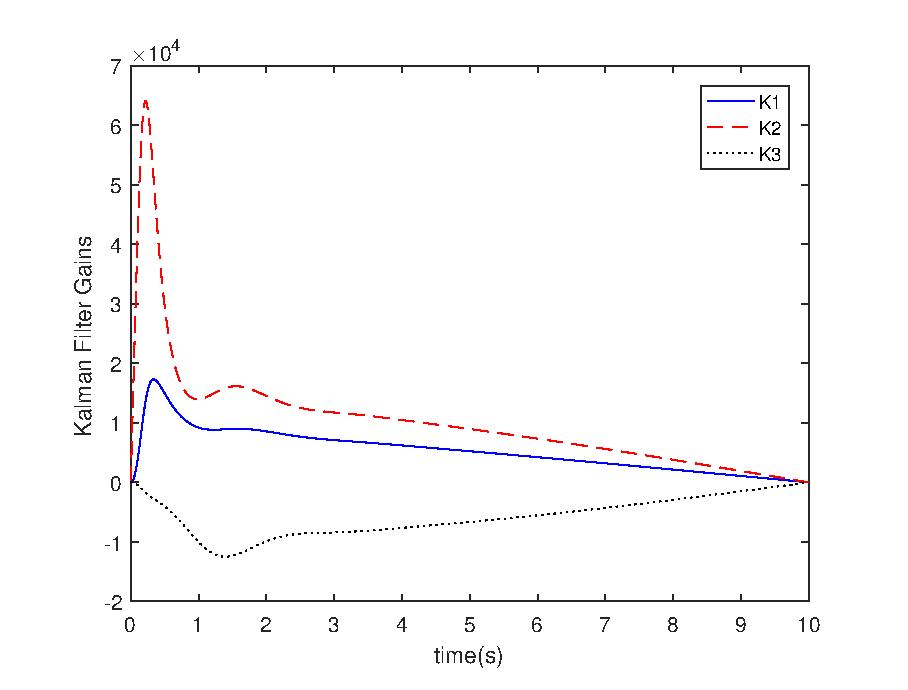
\includegraphics[width =0.8\textwidth]{Kgain}
	\caption{\textit{Filter Gain History}}
\end{figure}
\begin{figure}[H]
	\centering
	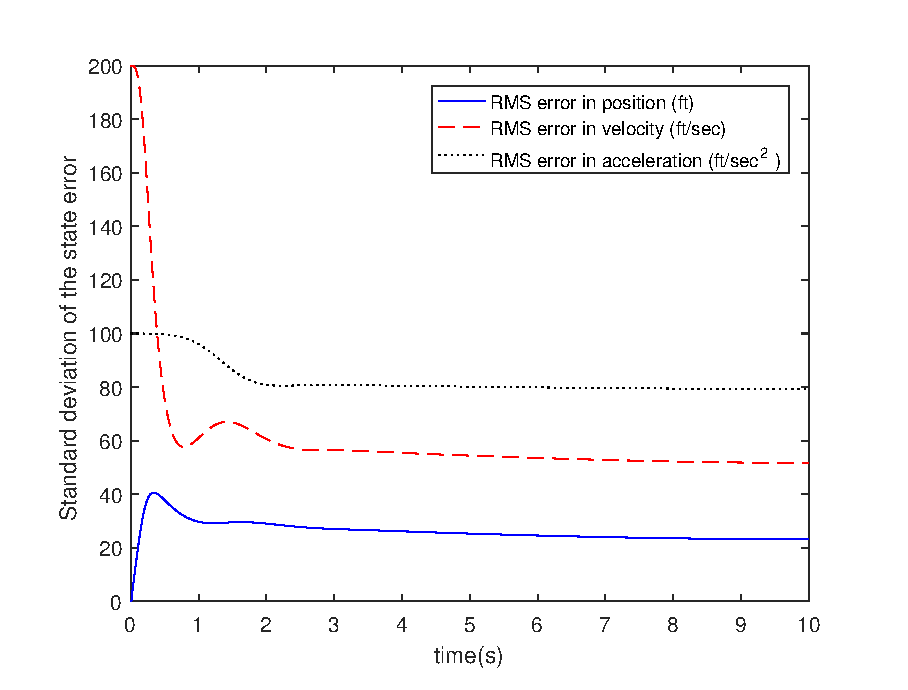
\includegraphics[width =0.8\textwidth]{errp}
	\caption{\textit{Evolution of the Estimation Error RMS}}
\end{figure}
\begin{figure}[H]
	\centering
	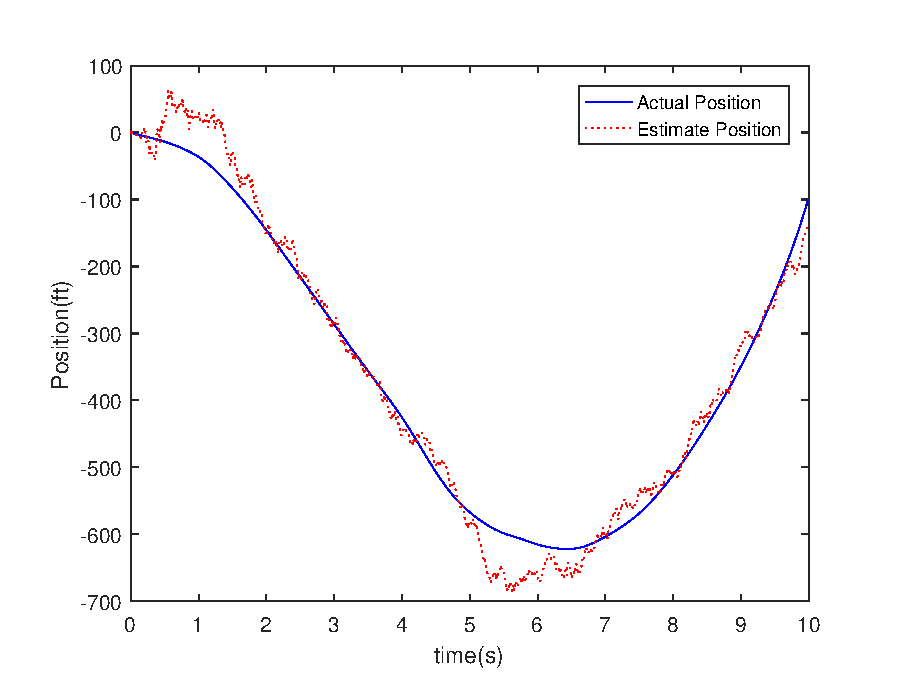
\includegraphics[width =0.8\textwidth]{po}
	\caption{\textit{Actual Position v.s. Estimate Position}}
\end{figure}
\begin{figure}[H]
	\centering
	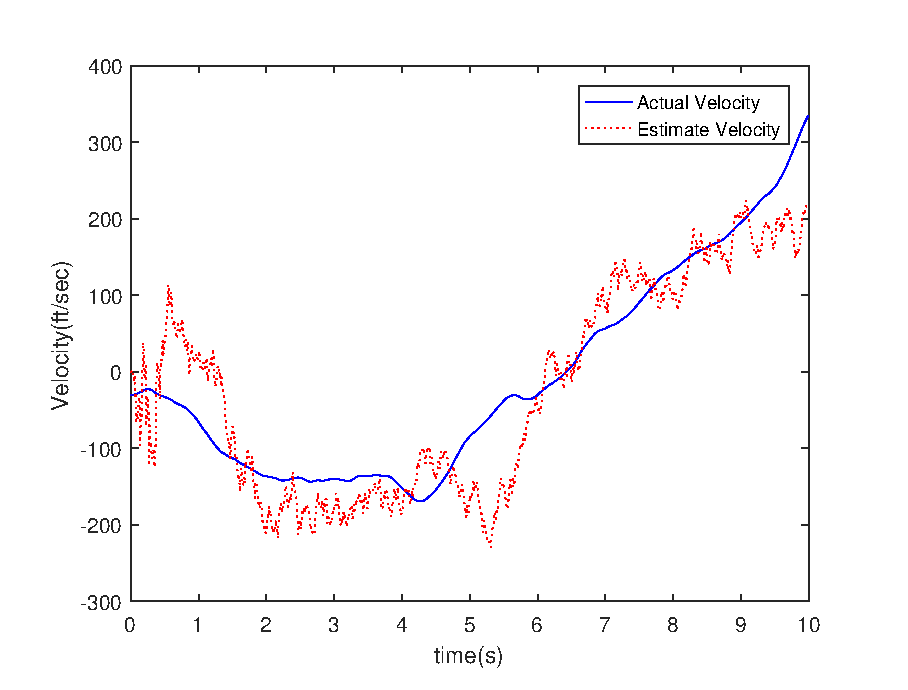
\includegraphics[width =0.8\textwidth]{vo}
	\caption{\textit{Actual Velocity v.s. Estimate Velocity}}
\end{figure}
\begin{figure}[H]
	\centering
	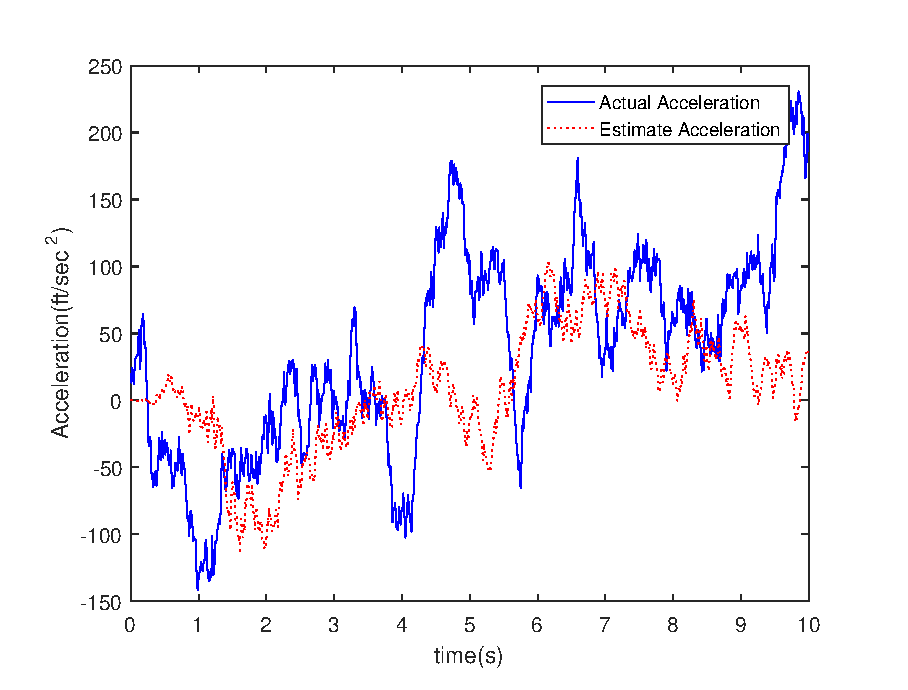
\includegraphics[width =0.8\textwidth]{ac}
	\caption{\textit{Actual Acceleration v.s. Estimate Accleration}}
\end{figure}
\begin{figure}[H]
	\centering
	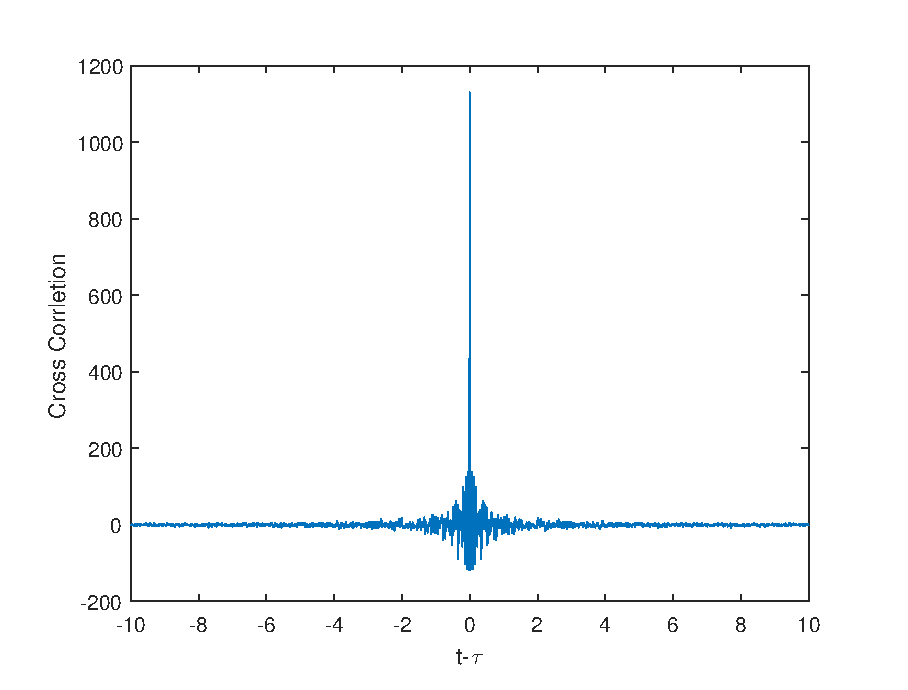
\includegraphics[width =0.8\textwidth]{corr}
	\caption{\textit{Cross Correlation of the Residue Process}}
\end{figure}
\subsubsection{Monte Carlo Analysis}
For the second part of the implementation, we show by a Monte Carlo simulation, the actual error variance matches the \textit{a priori} variance with 3 different sizes $N = 10,\ 100,\ 1000$ respectively. The error is defined as follows.
\begin{align*}
e =x-  \hat{x} 
\end{align*}
\paragraph{}
Figure 8-10 presents the ensemble average of the position, velocity and acceleration marked in red full line (due to lack of space, no legend is shown), bracketed by one-sigma bound of the \textit{a priori} variance. The ensemble average is calculated as follows. 
\begin{align*}
e^{ave}(t_i) = \frac{1}{N}\sum^N_{j = 1}e^j(t_i).
\end{align*}
\paragraph{}
Figure 11-14 shows a comparison between actual error variance and \textit{a priori} variance. As the number of realization increases, difference between the actual variance calculated and \textit{a priori} variance shrinks. The variance is calculated as follows.
\begin{align*}
P^{ave}(t_i)= \frac{1}{N-1}\sum_{j =1}^{N}[e^j(t_i)-e^{ave}(t_i)][e^j(t_i)-e^{ave}(t_i)]^T
\end{align*}
\begin{figure}[H]
	\centering
	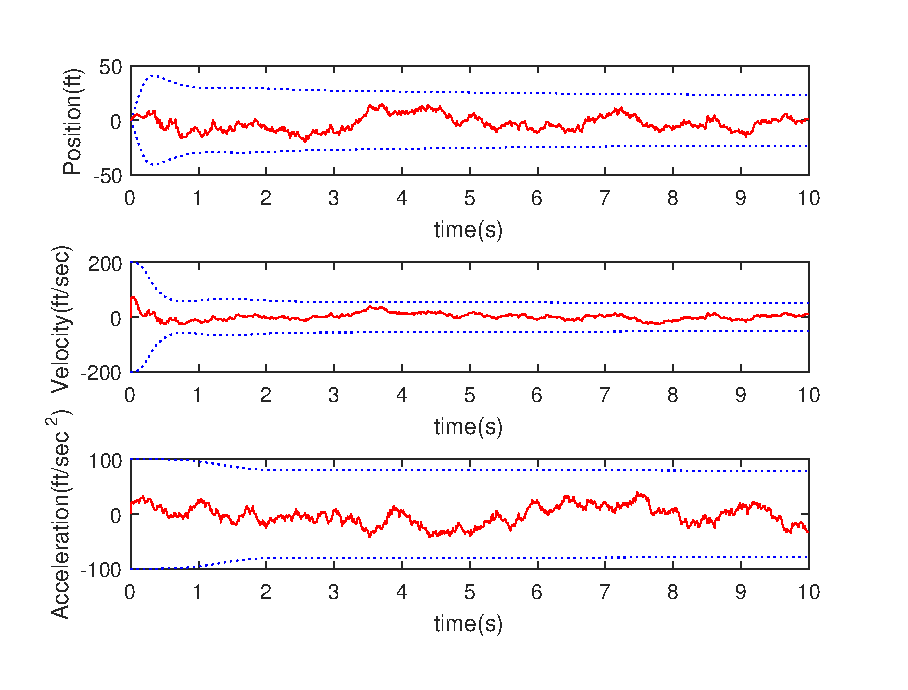
\includegraphics[width =0.8\textwidth]{en3}
	\caption{\textit{Ensemble Average of the states with N = 10}}
\end{figure}
\begin{figure}[H]
	\centering
	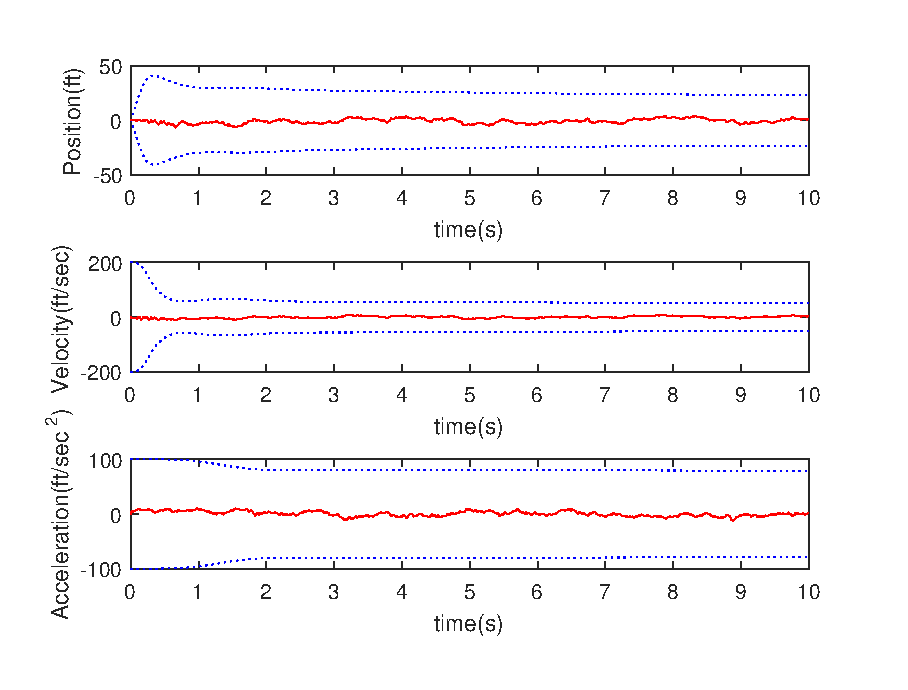
\includegraphics[width =0.8\textwidth]{en32}
	\caption{\textit{Ensemble Average of the states with N = 100}}
\end{figure}
\begin{figure}[H]
	\centering
	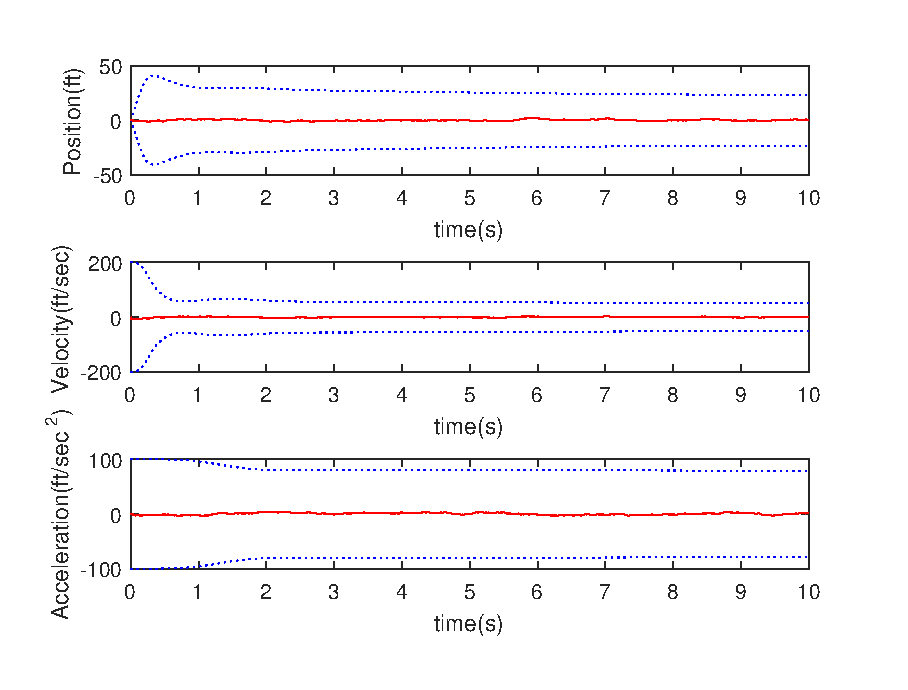
\includegraphics[width =0.8\textwidth]{en33}
	\caption{\textit{Ensemble Average of the states with N = 1000}}
\end{figure}
\begin{figure}[H]
	\centering
	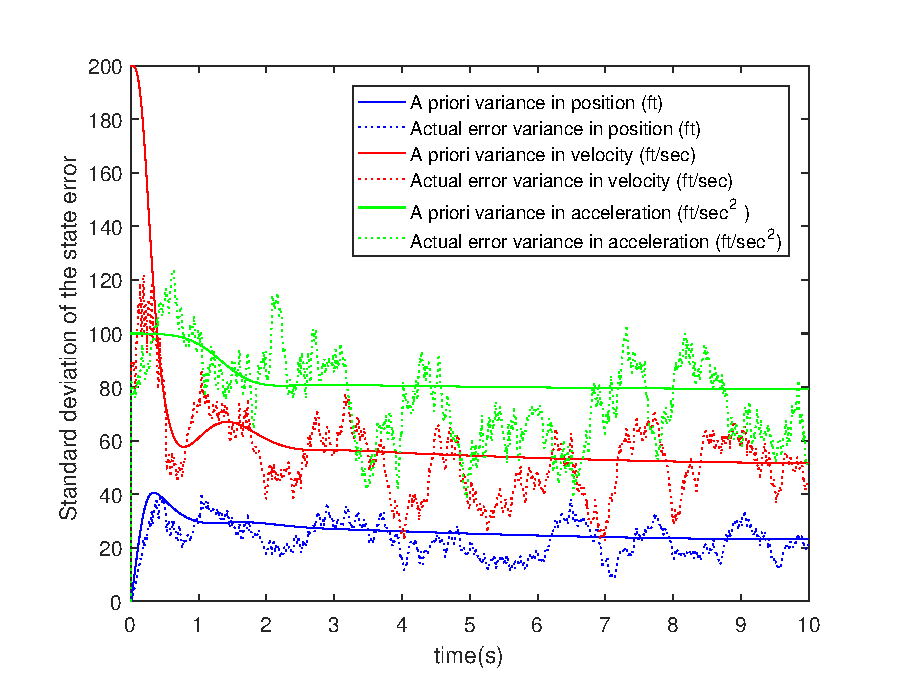
\includegraphics[width =0.8\textwidth]{en1}
	\caption{\textit{Actual Error Variance v.s. A Priori Variance with N = 10}}
\end{figure}
\begin{figure}[H]
	\centering
	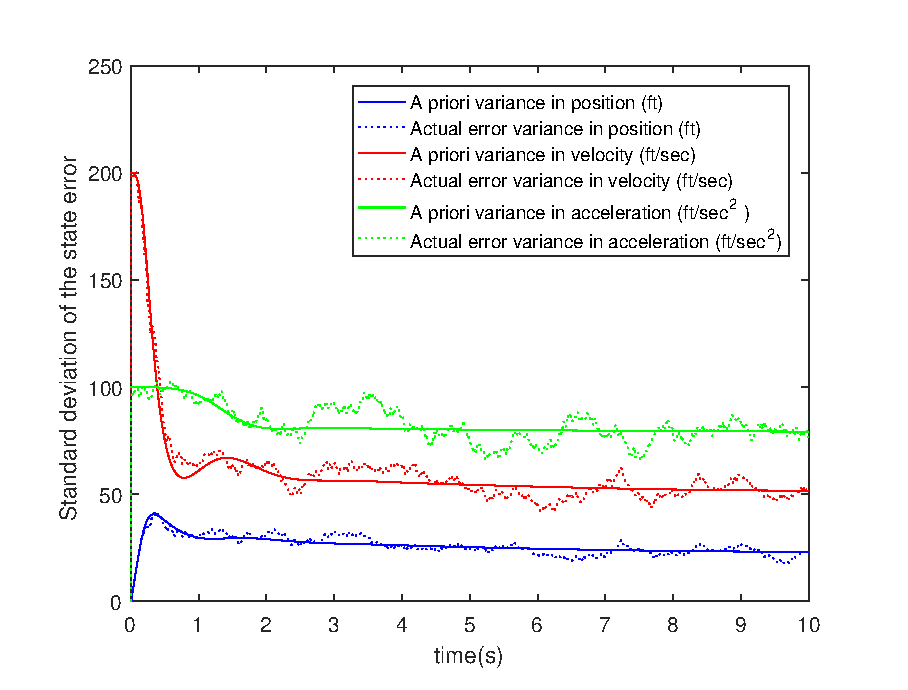
\includegraphics[width =0.8\textwidth]{en12}
	\caption{\textit{Actual Error Variance v.s. A Priori Variance with N = 100}}
\end{figure}
\begin{figure}[H]
	\centering
	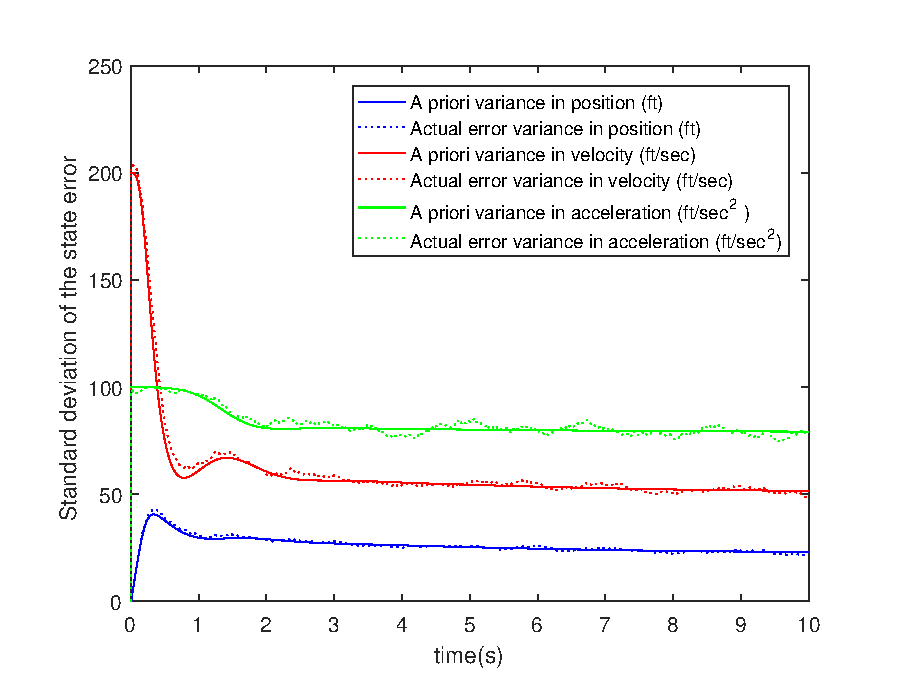
\includegraphics[width =0.8\textwidth]{en13}
	\caption{\textit{Actual Error Variance v.s. A Priori Variance with N = 1000}}
\end{figure}
\subsubsection{Random Telegraph Signal Model}
\paragraph{}
Recall that we made a few approximation when implementing the Kalman filter. Now we utilize a random telegraph signal, or \textit{Burst Noise}, to verify that the Kalman filter has been implemented corrected this way. In this model, the value $a_T$ changes sign at random times given by a \textit{Poisson} probability, defined as follows.
\begin{align*}
t_{n+1} = t_n - \frac{1}{\lambda}\ln(U),
\end{align*}
\paragraph{}
where $U$ is the output of $[0,1]$ uniform distribution and $\lambda = 0.25$. A single realization of $a_T$ is shown in Figure 14.
\begin{figure}[H]
	\centering
	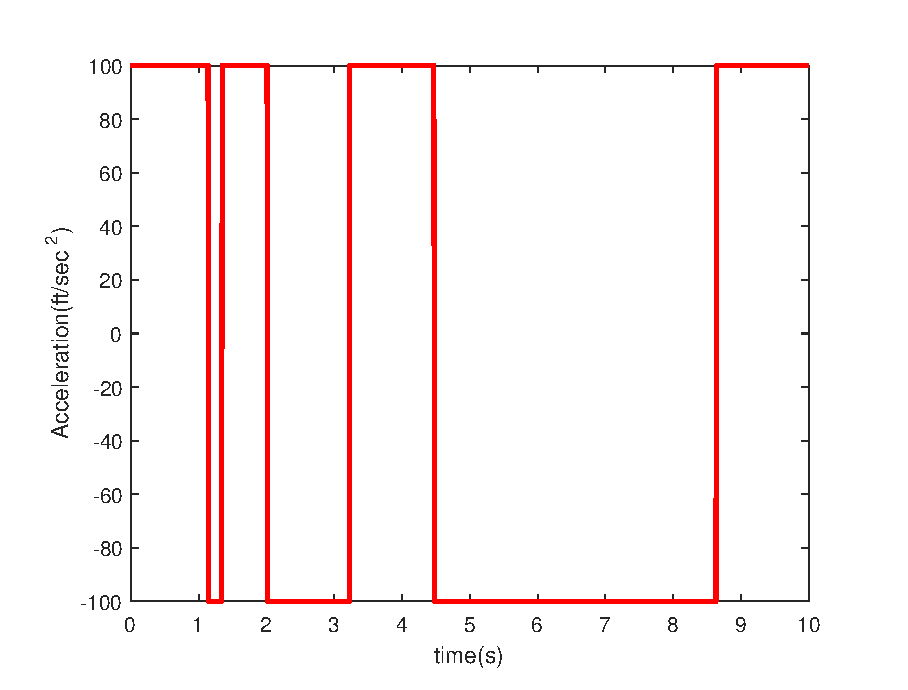
\includegraphics[width =0.8\textwidth]{acc}
	\caption{\textit{Single Realization of Acceleration Input using Random Telegraph Signal Model}}
\end{figure}
\paragraph{}
Essentially, we replaced the system input generated by a \textit{Gauss-Markov} process with a model described above and run Monte Carlo Simulation based on such input. Again, we have $N = 10,\ 100,\ 1000$ respectively. The results are shwon in Figure 15-20. As shown in Figure 15-17, as sample size $N$ increases, then ensemble average converges to zero, and in Figure 18-20, the actual error variance converge to \textit{a priori} variance.
\vspace{-12pt}
\paragraph{}
One interesting observation made during the implementation of the random telegraph signal is that the initial acceleration, instead of be selected randomly between $a_0 \text{ and } -a_0$, is set to a fixed value and therefore the Monte Carlo analysis results in a difference (less) in ensemble mean and variance in early stage, i.e, when $t$ is small. It converges to zero at steady state. At the beginning, it was believed to be some property of the random telegraph signal. However, this was a pure implementation error, and such less in statistics make sense since the beginning of the stage is deterministic and therefore there is less variance.

\begin{figure}[H]
	\centering
	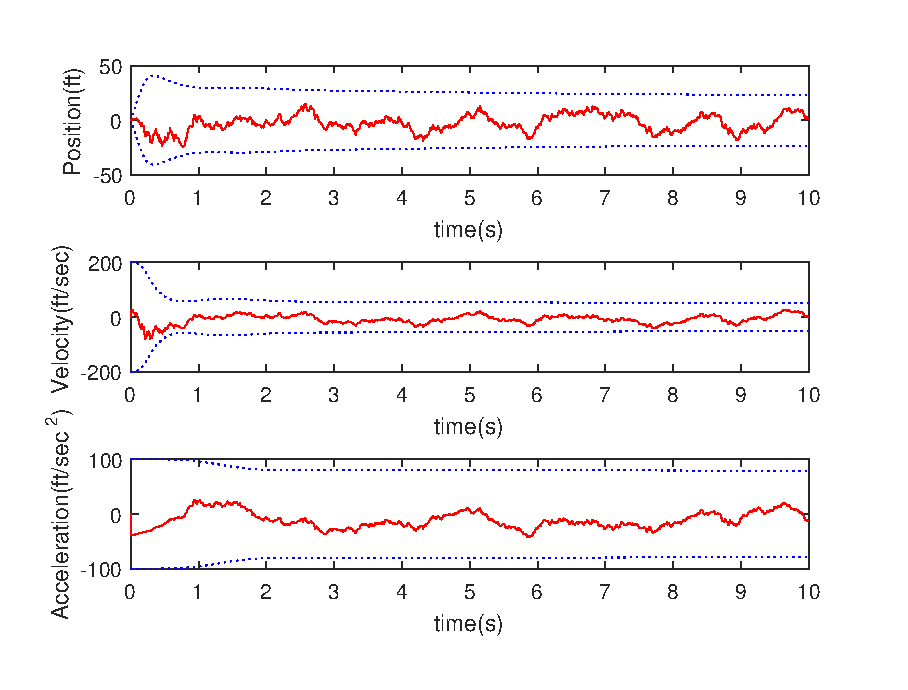
\includegraphics[width =0.8\textwidth]{t31}
	\caption{\textit{Ensemble Average of the states with N = 10}}
\end{figure}
\begin{figure}[H]
	\centering
	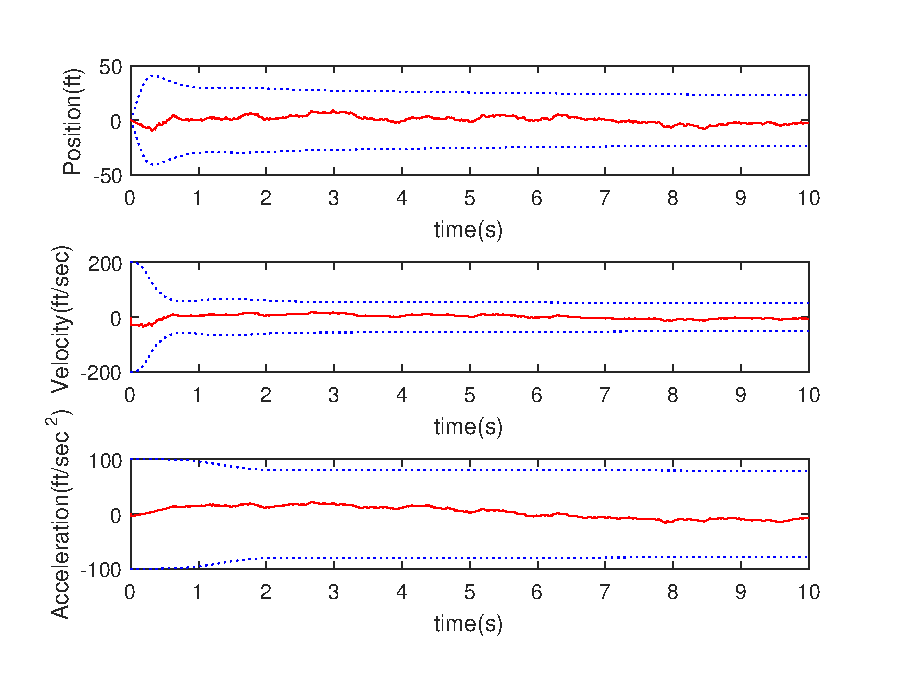
\includegraphics[width =0.8\textwidth]{t32}
	\caption{\textit{Ensemble Average of the states with N = 100}}
\end{figure}
\begin{figure}[H]
	\centering
	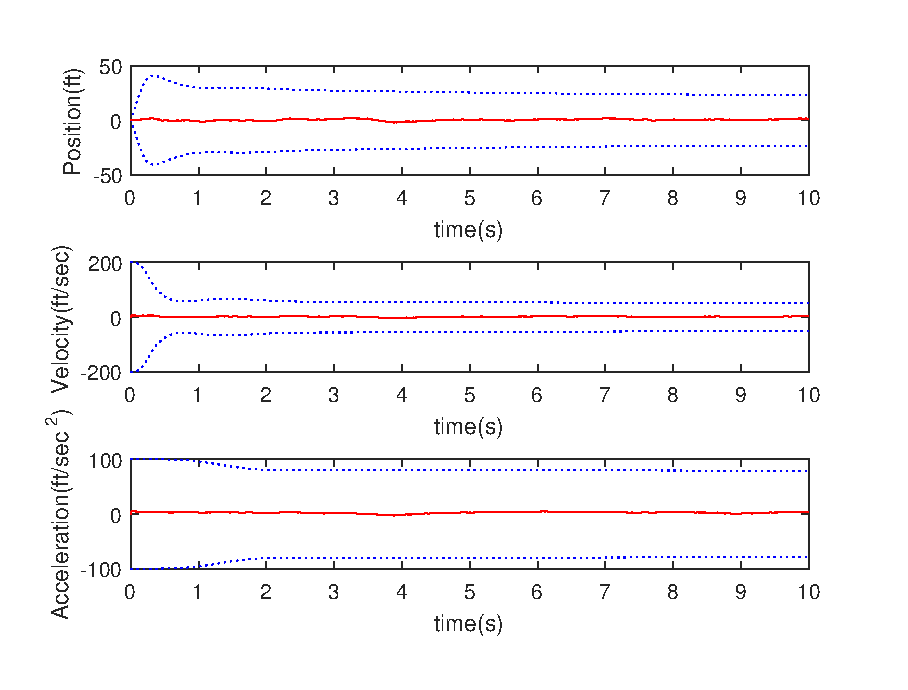
\includegraphics[width =0.8\textwidth]{t33}
	\caption{\textit{Ensemble Average of the states with N = 1000}}
\end{figure}
\begin{figure}[H]
	\centering
	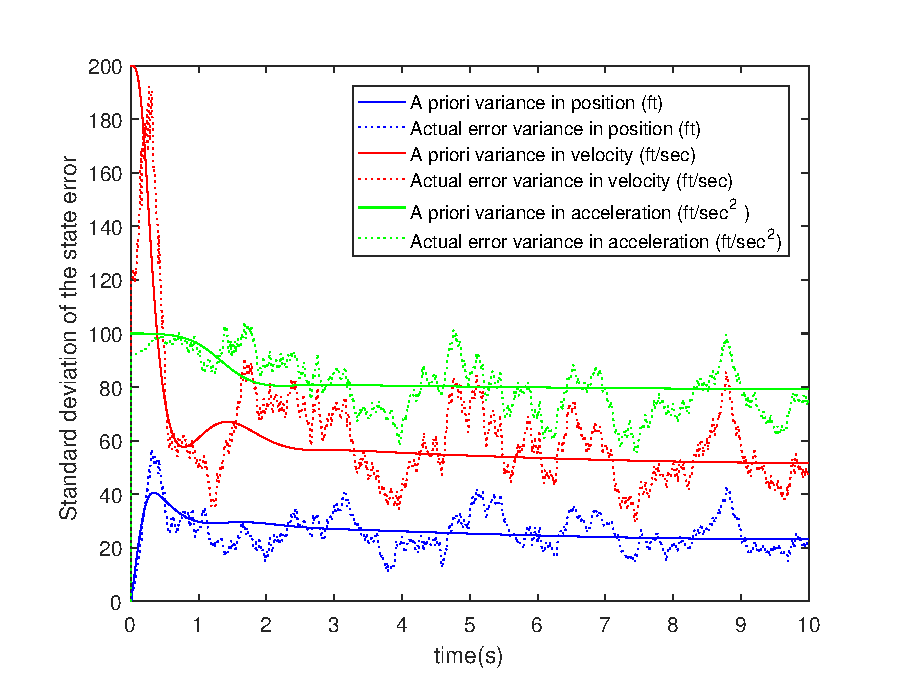
\includegraphics[width =0.8\textwidth]{t11}
	\caption{\textit{Actual Error Variance v.s. A Priori Variance with N = 10}}
\end{figure}
\begin{figure}[H]
	\centering
	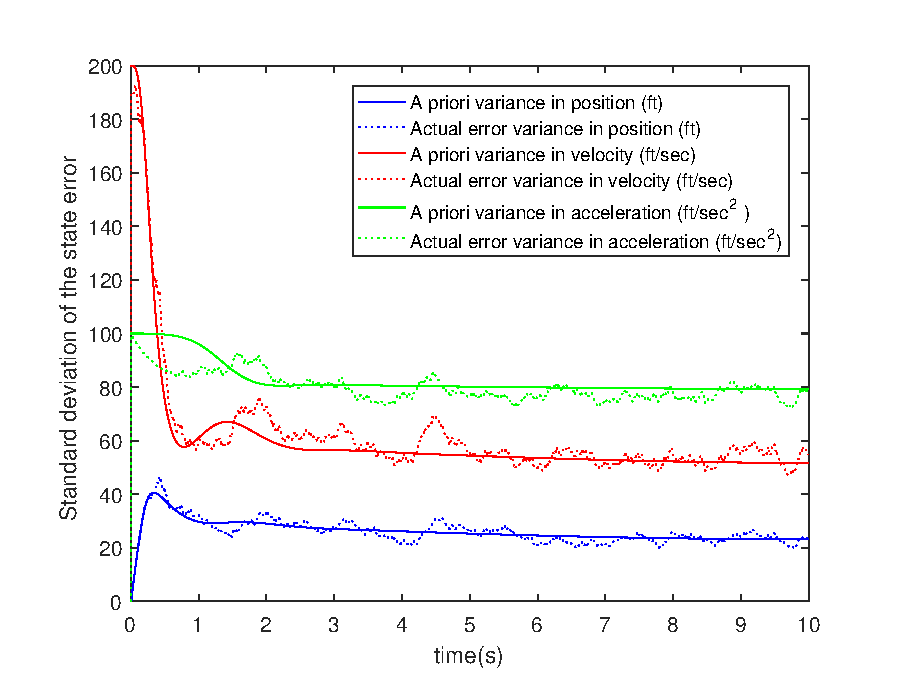
\includegraphics[width =0.8\textwidth]{t12}
	\caption{\textit{Actual Error Variance v.s. A Priori Variance with N = 100}}
\end{figure}
\begin{figure}[H]
	\centering
	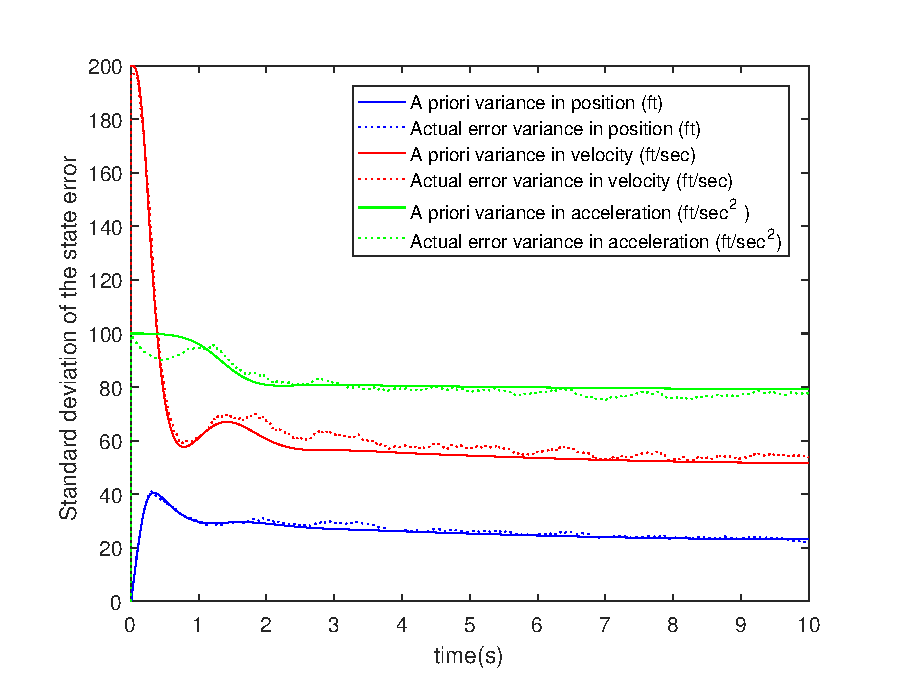
\includegraphics[width =0.8\textwidth]{t13}
	\caption{\textit{Actual Error Variance v.s. A Priori Variance with N = 1000}}
\end{figure}	